\subsection{NVM 星云链虚拟机}
\label{sec:nvm}

我们将引入LLVM~\cite{llvm}做为NVM的核心组件,LLVM byte code做为NVM字节码。NVM字节码通过LLVM JIT完成动态编译和优化,运行在NVM沙盒环境中。在这种架构设计下,星云链的核心代码、智能合约能直接享受到LLVM带来的性能和安全性的不断提升。

LLVM早期是Low Level Virtual
Machine的缩写,是一系列高度模块化的编译器和工具链技术的集合,包括Google、Apple在内的公司都使用它做为代码编译框架。LLVM提供了一套中立的中间表示(LLVM
IR)和相应的编译基础设施,并围绕这些设施提供了一套全新的编译策略,包括对LLVM
IR的优化、LLVM IR到不同硬件平台的代码生成、LLVM IR到LLVM byte
code的代码生成以及LLVM byte code在不同硬件平台上通过LLVM
JIT直接执行如图\ref{fig:llvm}所示

%LLVM编译框架分为三层,第一层支持多种语言作为输入(例如C/C++,go和python等),第二层是一个共享式的优化器(对LLVM IR做优化处理),第三层是许多不同的目标平台(例如 Intel, ARM和PowerPC),如图\ref{fig:llvm}所示

\begin{figure}[h]
\centering
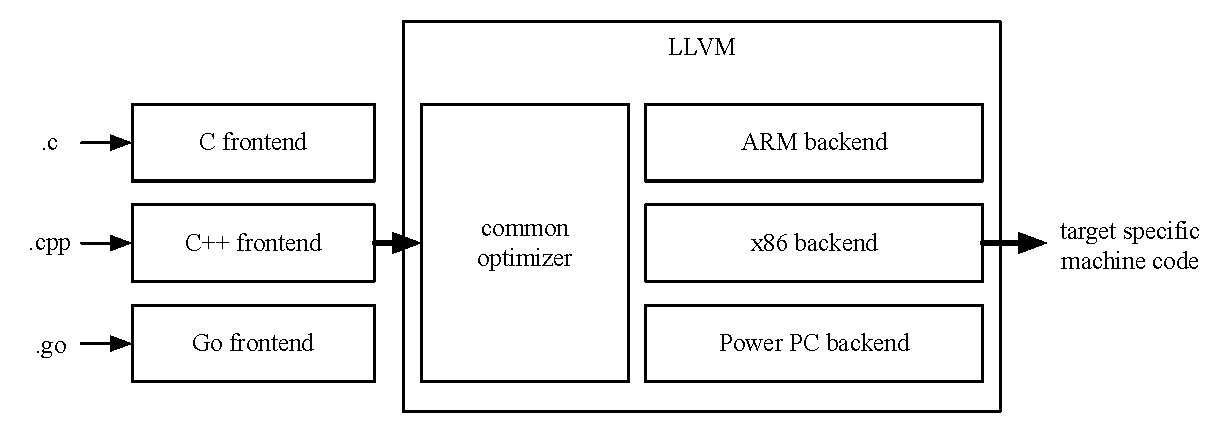
\includegraphics[width=10cm]{./figs/llvm}
\caption{LLVM}
\label{fig:llvm}
\end{figure}

我们依托LLVM构建NVM,如图\ref{fig:nvm}所示。首先,我们提供区块链底层API库;然后,我们为不同语言(如Solidity,Javascript
,C/C++,Go等)构建生成LLVM
IR的编译器前端,最后,利用LLVM提供的工具链,生成LLVM byte code。最终,LLVM byte
code通过LLVM的JIT引擎运行在NVM提供的安全的沙箱环境中。
%然后,利用LLVM链接器链接我们提供的底层库,LLVM
%JIT完成核心协议和智能合约代码的编译、优化以及跨平台适配,生成机器代码;最后,让这些机器代码通过LLVM的JIT引擎运行在NVM提供的安全的沙箱环境中。

\begin{figure}[h]
\centering
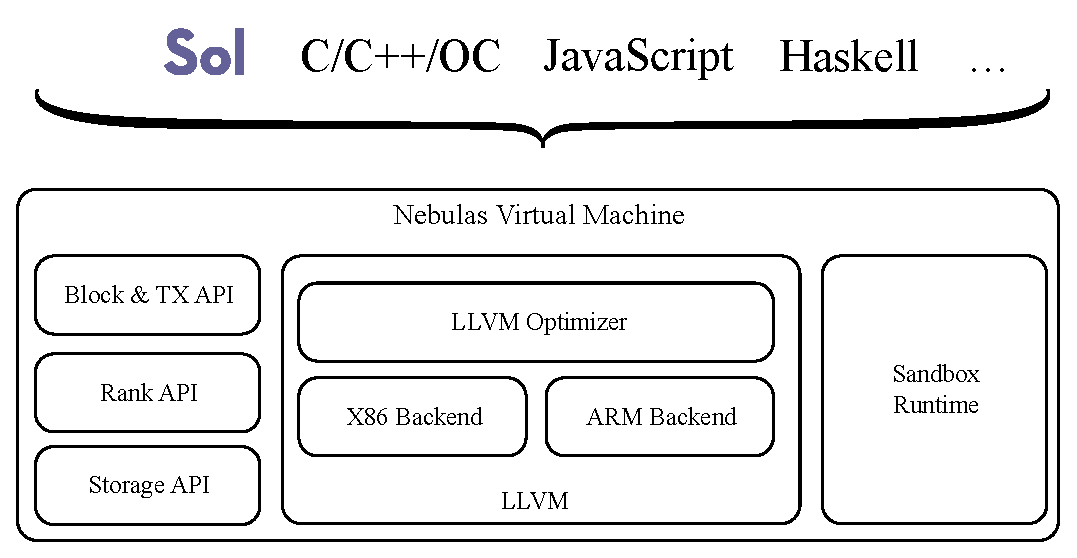
\includegraphics[width=10cm]{./figs/nvm}
\caption{星云链虚拟机}
\label{fig:nvm}
\end{figure}

NVM是星云原力的重要基石。新的协议代码或智能合约发布时,NVM中LLVM编译器模块完成新代码的编译得到LLVM字节码,然后发布到链上;链上确认后,新代码将由LLVM
JIT完成编译和优化,然后进入沙箱取代旧代码并被执行,过程如图\ref{fig:nvm-process}所示。 \\

\begin{figure}[h]
\centering
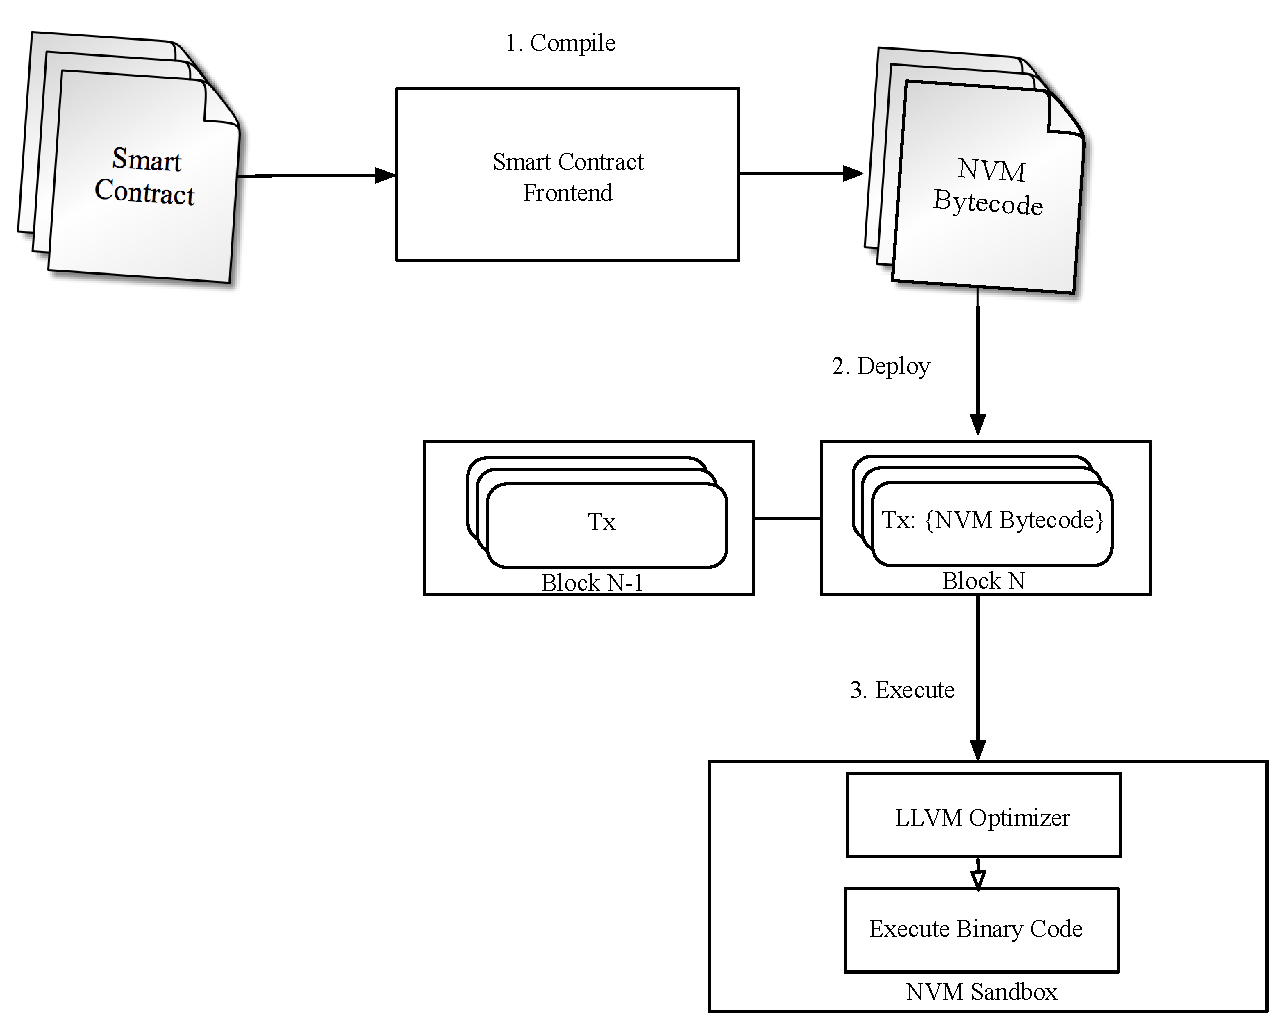
\includegraphics[width=10cm]{./figs/nvm-process}
\caption{星云链虚拟机运行机制}
\label{fig:nvm-process}
\end{figure}

借助于LLVM(见\ref{fig:llvm}),NVM还支持开发者用其熟悉的编程语言开发智能合约和应用,比如以太坊智能合约所使用的Solidity,更加灵活的JavaScript,甚至是纯函数式语言Haskell。除了这些通用语言外,NVM还可以为不同领域和场景提供定制的高级语言,比如面向金融行业的DSL(领域专有语言)。这类高级语言面向行业、场景高度定制,使得它们更容易被形式化验证,能进一步提高代码健壮性和安全性,更有利于星云链开发者开发出更丰富的智能合约及应用。
